\documentclass{article}
\usepackage{graphicx} % Required for inserting images
\usepackage{amsmath, bm, mathtools, amsfonts, amssymb}
\usepackage{xcolor}
\usepackage{adjustbox} 
\usepackage{hhline}
\usepackage{caption}
\usepackage[]{hyperref}
\captionsetup[table]{position=bottom} 
\usepackage{array, makecell}
\newcommand*{\vertbar}{\rule[-1ex]{0.5pt}{2.5ex}}
\newcommand*{\horzbar}{\rule[.5ex]{2.5ex}{0.5pt}}
\newcommand{\diff}{\mathop{}\!\mathrm{d}}

\usepackage{tikz}
\usetikzlibrary{decorations.pathreplacing,calligraphy}
\usetikzlibrary{positioning}
\usetikzlibrary{positioning,shapes.symbols,fit}
\tikzset{
	roundnode2/.style={circle, draw=green!50!blue, very thick, minimum size=9mm}
}
%\usetikzlibrary{shapes, arrows, calc, arrows.meta, fit, positioning}
%\usetikzlibrary{arrows.meta}
\tikzset{
	roundnode/.style={circle, draw=green!50!blue, fill=green!60!blue, very thick, minimum size=7mm},
	rectnode/.style={rectangle, draw=green!50!blue, very thick, minimum size=8.5mm},
	mydotted/.style = {dash pattern=on 6.1pt off 7pt}
}


%\usepackage[backend=bibtex,style=numeric,natbib=true,maxbibnames=5,giveninits=true]{biblatex}
\usepackage[backend=bibtex,style=numeric,natbib=true,maxbibnames=5,giveninits=true]{biblatex}

\newcommand*{\bibtitle}{References}
\DeclareNameAlias{default}{last-first}
%\DeclareSortingNamekeyTemplate{
%	\keypart{
%		\namepart{family}
%	}
%	\keypart{
%	\namepart{prefix}
%}
%	\keypart{
%		\namepart{given}
%	}
%	\keypart{
%		\namepart{suffix}
%	}
%}
%\renewbibmacro{begentry}{\midsentence}

\addbibresource{bib.bib}

\title{Tensor-Train Paper}
\author{Lennart}
\date{November 2025}
%\makeatletter
%\AtBeginDocument{\toggletrue{blx@useprefix}}
%\makeatother
\begin{document}

\maketitle
\begin{abstract}
	The radiative transfer equation (RTE) for a stratospheric limb-sounder measuring thermal radiation of ozone presents a weakly non-linear forward map.
Given some simulated data, this paper presents a hierarchical Bayesian framework to infer pressure, temperature and ozone concentration values and some other hyper-parameters such as the noise covariance and the ozone smoothness.
Thereby the non-linear forward model is approximated with an affine map and the linearised RTE, which in combination with the marginal-then-conditional scheme~\cite{fox2016fast} and a tensor-train approximation of the marginal posterior over the hyper-parameters enables efficient inference.
\end{abstract}

\section{Introduction}
There are satellites, which orbit around the earth at a height of around 500km above the ground, that carry measurement devices to determine trace gas concentrations in the stratosphere.
More specifically, atmospheric limb-sounders are pointing through the atmosphere and detect thermal radiation of trace gases, e.g., ozone.
Examples of such limb-sounders are the Microwave
Limb Sounder (MLS) on NASA’s Aura mission~\cite{waters2006earth} and the
Michelson Interferometer for Passive Atmospheric Sounding
(MIPAS) on ESA’s Envisat~\cite{readings2000envisat}.

Measurements of such devices can be described by the radiative transfer equation (RTE), which in this case is a path integral along the satellite's pointing direction.
This path integral includes an absorption term accounting for the re-attenuation of the thermal radiation along the satellite's line of sight.
That makes inferring the trace gas concentration from a set of measurements a non-linear inverse problem.

Existing frameworks use regularisation methods to retrieve trace gas concentration from measurements~\cite{rodgers1976retrieval, livesey2006retrieval, raspollini2021level}.
These methods do not include hyper-parameters, such as noise covariance, and produce biased results~\cite{Froidevaux2008snrozone}.
Additionally, atmospheric states such as pressure and temperature are retrieved from some previous measurements.
Conditioned on those estimates further analysis is carried out to, e.g., retrieve ozone concentrations \cite{livesey2006retrieval,EOSMLSRetrival2004}.

In this paper, we develop a framework where pressure and temperature are treated as unknowns and are included within the modelling and inversion process.
In doing so, the pressure and temperature profile is parametrised, whereas a non-parametric model for the ozone is used.
Firstly, given some simulated data, we treat this non-linear problem as a linear problem by neglecting the absorption term in the RTE.
A linear-Gaussian hierarchical Bayesian framework is employed to infer the ozone concentration in the stratosphere and to provide pressure and temperature values.
This includes establishing a hierarchical structure and classifying hyper-parameters and parameters.
For efficient inference we employ the marginal-then-conditional (MTC) scheme as in~\cite{fox2016fast} and extend it to include model describing hyper-parameters related to pressure and temperature.
This gives a marginal posterior probability distribution over the hyper-parameters and a high-dimensional conditional posterior probability for the ozone parameter.
We show that approximating the marginal posterior on a grid using a functional tensor-train (TT) is an efficient alternative to conventional sampling-based methods to generate hyper-parameter samples from the marginal posterior.
Conditioned on hyper-parameter samples, ozone samples from the full conditional posterior are drawn via the randomise-then-optimise (RTO) scheme~\cite{bardsley2012mcmc}.
Using the results of the linearised problem, an affine map approximating the non-linear forward model is obtained.
We employ the same hierarchical Bayesian framework as previously used, but with the approximated forward model, to quantify the posterior mean and variance of pressure, temperature and ozone.

All programming and analysis in this paper are done in Python, and the reported computation times are taken on a MacBook Pro from 2019 with a 2.4 GHz quad-core Intel i5 processor.
The code will be/is available here: \url{https://deeptransport.github.io/deep-tensor-py/examples/}.



%\begin{itemize}
%	\item Hierarchical Bayesian modelling including Pressure and Temperature
%	\item parametrised model for pressure and temperature and non-parametric model for ozone
%    \item Forward model ozone limb-sounding as linear inverse problem
%    \item Marginal and full conditional posterior explicitly formulated
%    \item samples from full conditional posterior via IRT
%    \item sample-based affine map
%    \item same procedure again
%    \item full posterior mean and sample-based variance do not capture second ozone peak
%    \item Pressure and Ozone highly correlated
%    \item All programming and analysis in this thesis are done in Python, and the reported computation times are taken on a MacBook Pro from 2019 with a 2.4 GHz quad-core Intel i5 processor.
%    \item \url{https://deeptransport.github.io/deep-tensor-py/examples/}
%\end{itemize}
\section{Hierarchical Bayesian Modelling}
\label{sec:BayesIntro}
First, the concept of hierarchical Bayesian modelling is introduced.
Assume we observe some data
\begin{align}
	\bm{y} = \bm{A}( \bm{x}) + \bm{\eta},
	\label{eq:NonLinDat}
\end{align}
based on the forward model $\bm{A}(\bm{x})$ with an unknown parameter vector $\bm{x}$ and some additive random noise $\bm{\eta}$.
Naturally, due to the noise, the observation process in Eq. \ref{eq:NonLinDat} is a random process.
Hence, in Bayesian modelling, the aim is to determine a probability distribution over the parameter $\bm{x}$ given some data $\bm{y}$.
Further, a hierarchical Bayesian model incorporates (auxiliary) hyper-parameters $\bm{\theta}$ (see Fig.~\ref{fig:FirstDAG} for a schematic representation).
Within a Bayesian approach all unknown hyper-parameters and parameters are treated as random variables~\cite[Chapter 3]{kaipio2005statinv}.
\begin{figure}[ht!]
	\centering
	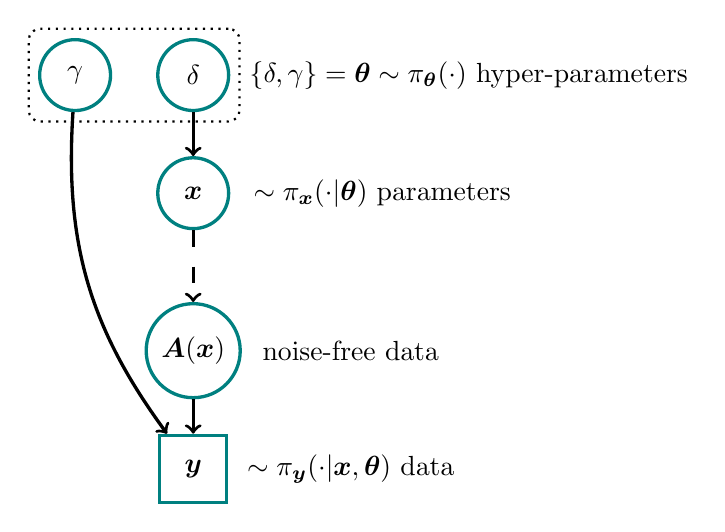
\begin{tikzpicture}
		
		every edge/.style = {draw, -latex, thick} % <---
		\node[roundnode2] at (0,2) (del)    {$\delta$};
		\node[roundnode2] at (-1.5,2) (gam)    {$\gamma$};
		%\node[align=center] at (-0.75,2.25) (theta) {$\bm{\theta}$};
		\node[roundnode2] at (0,0.5) (x)    {$\bm{x}$};
		\node[roundnode2] at (0,-1.5) (u)    {$\bm{A}(\bm{x})$};
		\node[rectnode] at (0,-3) (y)    {$\bm{y}$};
		
		%\node[align=center] at (-3.25,0) (nt) {noise\\$\bm{\eta} \sim$};
		
		\draw[->, very thick, mydotted] (x.south) -- (u.north); 
		\draw[->, very thick] (u.south) -- (y.north); 
		\draw[->, very thick] (del.south) -- (x.north); 
		\draw[->, very thick] (gam) edge[bend right=20] (y);  
		
		\node[align=center] at (3.5,2) (tht) {$\{\delta, \gamma\} = \bm{\theta}\sim \pi_{\bm{\theta}}(\cdot) $ hyper-parameters};
		\node[align=center] at (2.4,0.5) (xt) {$\sim \pi_{\bm{x}}(\cdot|\bm{\theta}) $ parameters};
		\node[align=center] at (2,-1.5) (ut) {noise-free data};
		\node[align=center] at (2,-3) (yt) {$\sim \pi_{\bm{y}}(\cdot|\bm{x},\bm{\theta})$ data};
		%\node[align=center] at (-3.25,0) (nt) {noise\\$\bm{\eta} \sim \pi_{\bm{\eta}}(\cdot|\bm{\theta})$};
		%\node[fit=(s)(d),draw,dotted,black, rounded corners] {};
		\node[fit=(del)(gam),draw,thick,dotted,black, rounded corners] {};
	\end{tikzpicture}
	\caption[Hierarchical Bayesian Model]{\textcolor{red}{A directed acyclic graph (DAG) for an inverse problem visualises statistical dependencies as solid line arrows and deterministic dependencies as dotted arrows.
			The hyper-parameters $\bm{\theta}$ are distributed as ($\sim$) the hyper-prior distribution $\pi(\bm{\theta})$.
			The prior distribution $ \pi_{\bm{x}}(\cdot|\bm{\theta})$ for the parameter $\bm{x}$ and the noise  $\bm{\eta} \sim \pi_{\bm{\eta}}(\cdot|\bm{\theta})$ are statistically dependent on some of those hyper-parameters.
			Then a parameter $\bm{x} \sim \pi_{\bm{x}}(\cdot|\bm{\theta})$ is deterministically mapped through the forward model $\bm{A}(\bm{x})$.
			Based on the noise-free data we observe (square box) a data set $\bm{y} = \bm{A}(\bm{x}) + \bm{\eta}$ with some additive random noise, which determines the likelihood function $\pi(\bm{y}|\bm{x},\bm{\theta})$.}}
	\label{fig:FirstDAG}
\end{figure}

According to Bayes' theorem, the joint posterior distribution over the parameters $\bm{x}$ and the hyper-parameter $\bm{\theta}$ is given as
\begin{align}
	\pi(\bm{x},\bm{\theta}|\bm{y}) = \frac{ \pi(\bm{y} | \bm{x}, \bm{\theta} ) \pi(\bm{x}, \bm{\theta})}{\pi(\bm{y})} \propto \pi(\bm{y} | \bm{x}, \bm{\theta} ) \pi(\bm{x}, \bm{\theta}) \, ,
\end{align}
with finite and non-zero $\pi(\bm{y})$.
The likelihood function $\pi(\bm{y}|\bm{x},\bm{\theta})$ is defined by the nature of the noise and the noise-free data $\bm{A}(\bm{x})$, which we read as the distribution over $\bm{y}$ conditioned on $\bm{x}$ and $\bm{\theta}$.
Here $\bm{\theta}$ describe multiple hyper-parameters, e.g.~the noise precision so that $\bm{\eta} \sim \pi_{\bm{\eta}}(\cdot|\bm{\theta})$, where $\sim$ reads as ``is distributed as''.
Further, $\bm{\theta}$ may account for some physical properties of $\bm{x}$ such as the smoothness (see Sec.~\ref{sec:BayModel}).
Because all unknown parameter are treated as random variables the joint prior distribution is introduced as $\pi(\bm{x}, \bm{\theta}) = \pi(\bm{x}|\bm{\theta}) \pi(\bm{\theta})$ with the parameter prior distribution $\pi(\bm{x}|\bm{\theta})$ and the hyper-prior distribution $\pi(\bm{\theta})$.
Choosing these prior distributions is ultimately a modeller's choice and is crucial, as those shall be as uninformative as possible for regions in hyper-parameter and parameter space where the data is informative.
If the data is uninformative, the prior distributions can be informative and may represent a rather restrictive range of (physically) feasible hyper-parameters and parameters.

We can write the hierarchical model as:
\begin{subequations}
	\begin{align}
		\bm{y} |  \bm{x},\bm{\theta}  &\sim \pi(\bm{y} | \bm{x}, \bm{\theta} ) \\
		\bm{x}| \bm{\theta}   &\sim \pi(\bm{x}|\bm{\theta})   \\
		\bm{\theta}   &\sim \pi(\bm{\theta} ) \, .
	\end{align} 
\end{subequations}
Usually, the objective is to calculate the expectation of a function $h(\bm{x})$, which is defined as
\begin{align}
	\text{E}_{\bm{x},\bm{\theta}|\bm{y}} [h(\bm{x})] =  \int \int   h(\bm{x}) \,  \pi(\bm{x}, \bm{\theta} | \bm{y} ) \, \diff \bm{x}  \, \diff \bm{\theta}  \label{eq:expPos} \, .
\end{align}
\subsection{Marginal-then-Conditional Method}
\label{subsec:TheoMTC}
Characterising the posterior distribution or quickly generating a representative sample set from the posterior distribution often presents a significant challenge. 
This is mainly due to the strong correlations that usually exist between the parameters $\bm{x}$ and hyper-parameters $\bm{\theta}$, as discussed by Rue and Held in~\cite{rue2005gaussian}.

Depending on the problem and the available model, it is beneficial to factorise the joint posterior distribution
\begin{align}
	\pi(\bm{x}, \bm{\theta} |  \bm{y}) = \pi(\bm{x} |  \bm{\theta}, \bm{y}) \, \pi(\bm{\theta} |   \bm{y}) \label{eq:MTC}
\end{align}
into the full conditional posterior $\pi(\bm{x} |  \bm{\theta}, \bm{y})$ over the latent field $\bm{x}$ and the marginal posterior $ \pi(\bm{\theta} |   \bm{y})$ over hyper-parameter $\bm{\theta}$.
This approach, known as the marginal-and-then-conditional (MTC) method~\cite{fox2016fast}, is particularly advantageous when $\bm{x}\in \mathbb{R}^n$ is high-dimensional, while $\bm{\theta}$ is low-dimensional and the evaluation of the marginal posterior
\begin{align}
	\pi(\bm{\theta} |   \bm{y}) =  \frac{ \pi(   \bm{y} | \bm{x},\bm{\theta})  \pi( \bm{x} | \bm{\theta} )  \pi(\bm{\theta}) }{ \pi(\bm{x} | \bm{\theta} ,   \bm{y})   \pi( \bm{y})} \propto \frac{ \pi(   \bm{y} | \bm{x},\bm{\theta})  \pi( \bm{x} | \bm{\theta} )  \pi(\bm{\theta}) }{ \pi(\bm{x} | \bm{\theta} ,   \bm{y}) } \label{eq:margGen}\, 
\end{align}
as in~\cite[Lemma 2]{fox2016fast} is relatively cheap.
Applying the law of total expectation~\cite{champ2022generalizedlawtotalcovariance}, Eq.~\eqref{eq:expPos} becomes
\begin{align}
	\mathbb{E}_{\bm{x} ,\bm{\theta}  |\bm{y}} [h(\bm{x})] &= \int \int   h(\bm{x}) \pi(\bm{x} |  \bm{\theta}, \bm{y}) \, \diff \bm{x} \,  \pi(\bm{\theta} |   \bm{y}) \, \diff \bm{\theta} \\
	&= \int \mathbb{E}_{\bm{x} |  \bm{\theta}, \bm{y}} \left[ h(\bm{x}) \right] \, \pi(\bm{\theta} |  \bm{y}) \, \diff \bm{\theta}\label{eq:2fullCond} \\
	&= \mathbb{E}_{\bm{\theta} |  \bm{y}} \left[ \mathbb{E}_{\bm{x} |  \bm{\theta}, \bm{y}} [h(\bm{x})] \right] \, .
	\label{eq:fullCond}
\end{align}

In the case of a linear-Gaussian hierarchical Bayesian model, both the marginal distribution $\pi (\bm{\theta}| \bm{y})$ 
and the inner expectation $\mathbb{E}_{\bm{x} |  \bm{\theta}, \bm{y}} \left[ h(\bm{x}) \right]$ are well defined (see Sec.~\ref{sec:BayModel} and \cite{fox2016fast}).
If the integral in Eq.~\ref{eq:2fullCond} is expensive to calculate sample-based methods may be used to calculate the expectations in 
Eq.~\eqref{eq:2fullCond}.
To produce samples $\{ (\bm{x}, \bm{\theta})^{(1)}, \dots, (\bm{x}, \bm{\theta})^{(k)}, \dots, (\bm{x}, \bm{\theta})^{(N)} \} \sim \pi(\bm{x}, \bm{\theta} |  \bm{y}) $ one needs an independent sample from $\bm{\theta}^{(k)} \sim \pi(\bm{\theta} |  \bm{y})$ first and then draws a sample from the full conditional posterior $\bm{x}^{(k)} \sim \pi(\bm{x} | \bm{\theta}^{(k)}  , \bm{y})$.

\textcolor{red}{
	Note that for the affine case, where e.g., the forward model is given by $\bm{A}\bm{x} + \bm{b}$, the MTC method as in \cite{fox2016fast} is still applicable.
	For Gaussian noise and a Gaussian prior, the form of the posterior of the affine case does not change compared to the linear-Gaussian case, where the forward model may be given by $\bm{A}\bm{x}$.}
\clearpage

\section{The Forward Model}
\label{ch:formodel}
Here we present the forward model to which we apply the methodology.
The forward model describes a Limb-sounder measuring thermal radiation of ozone to determine the atmospheric ozone concentration.
We follow the MIPAS handbook~\cite{mipas2000handbook} and simulate data according to an idealised cloud-free atmosphere in local thermodynamic equilibrium, assuming a measurement instrument with infinite spectral resolution and no pointing errors.
This is a simplified forward model.
No other instrument-specific details such as sensor area or antenna response are included because they are not available to us. 

\begin{figure}[ht!]
	\centering
	\input{LIMB.pdf_tex}
	\caption[Schematic of measurement and analysis geometry.]{Schematic of measurement and analysis geometry, not to scale.
		The stationary satellite, at a constant height $h_\text{sat}$ above Earth, takes $m$ measurements along its line-of-sight defined by the line $\Gamma_j$.
		Each measurement has a pointing angle $\phi_j$ and a tangent height $h_{\ell_j}$, $j=1,2,\dots,m$ defined as the closest distance of $\Gamma_j$ to the Earth's surface.
		Between $h_{L,0} \approx 7$km and $h_{L,n} \approx 83$km, the atmosphere is discretised into $n$ layers as illustrated by the solid green lines.}
	\label{fig:LIMB}
\end{figure}
As displayed in Fig.~\ref{fig:LIMB}, a satellite at a constant height $h_{\text{sat}}$ is pointing through the atmosphere (limb-sounding) to measure thermal radiation of ozone.
For each measurement $j=1,2,\ldots,m$, the tangent height $h_{\ell_j}$ and the corresponding line-of-sight $\Gamma_j$ are defined.
Additionally, we introduce the pointing angle $0 \leq \phi_j < \phi_{\text{max}}$, so that if $\phi = 0 \text{arc sec}$ the satellite points at $h_{L,0}$ and for a pointing angle $\phi_{\text{max}}$ at $h_{L,n}$.
Further, the atmosphere is discretised into $n$ layers defined by height values $h_{L,i-1} < h_{L,i}$ with respect to the surface of the Earth, for $i = 1, \dots, n$.
More specifically, the $i$-th layer is defined by two spheres around the centre of the Earth with radii $ r_0 + h_{L,i-1} $ and $r_0 + h_{L,i}$, where $r_0$ is the Earth's radius.
Within a layer the signal is constant, whereas above $h_{L, n}$ and below $h_{L,0} $ no signal can be obtained.


\subsection{Radiative Transfer Equation}
\label{sec:RTE}
One noise-free measurement of thermal radiation emitted by gas molecules within the atmosphere is described by the radiative transfer equation (RTE)~\cite{mipas2000handbook}
\begin{align}
	\label{eq:RTE} 
	  \int_{\Gamma_j}  B(\nu,T) k(\nu, T)   \frac{p(r)}{k_{\text{B}} T(r)}  x(r)  \tau(r) \text{d}r \,  \\
\text{with } \,	\tau(r) = \exp{ \Bigl\{ - \int^{r}_{r_\text{obs}}  k(\nu, T)   \frac{p(r^{\prime})}{k_B T(r^{\prime})}  x(r^{\prime}) \text{d}r^{\prime} \Bigr\} } \, \label{eq:absRTE} .
\end{align}
This is a path integral along the satellite's straight line of sight $\Gamma_j$ with the ozone volume mixing ratio (VMR) $x(r)$ at distance $r$ from the satellite, at the wave number $\nu$.
Within the atmosphere, the number density $p(r) / (k_{\text{B}} T(r))$ of molecules is dependent on the pressure $p(r)$, the temperature $T(r)$, and the Boltzmann constant $k_{\text{B}}$.
The factor $\tau(r)\leq 1$ accounts for re-absorption of the radiation along the line-of-sight, which makes the RTE non-linear.
The absorption constant is given as
\begin{align}
	k(\nu, T) = L(\nu, T_{\text{ref}}) \frac{Q(T_{\text{ref}})}{Q(T)} \frac{ \exp{\{ - c_2 E^{\prime \prime} / T\}} }{\exp{\{ - c_2 E^{\prime \prime} / T_{\text{ref}} \}}} \frac{ 1- \exp{\{ - c_2 \nu  / T \}} }{1 - \exp{\{ - c_2 \nu / T_{\text{ref}} \}}}
\end{align}
with Planck's constant $h$ and speed of light $c$.
The line intensity $L(\nu, T_{\text{ref}})$ at reference temperature $T_{\text{ref}} =296K $, the lower-state energy $ E^{\prime \prime} $ in $\text{cm}^{-1}$ of the targeted transition and the second radiation constant $c_2\coloneqq hc/k_{\text{B}} \approx 1.44\text{cmK}$ are provided by the HITRAN database~\cite{gordon2022hitran2020}.
The total internal partition function is given as
\begin{align}
	Q(T )= g^{ \prime} \exp{\{ - \frac{ c_2 E^{ \prime} }{T}\}} + g^{\prime \prime} \exp{\{ - \frac{ c_2 E^{\prime \prime} }{T}\}} \, ,
\end{align}
with the statistical weight $ g^{\prime \prime}$ for the lower and $ g^{ \prime}$ for the upper energy state (also called the degeneracy factors) accounting for the molecule's non-rotational and rotational energy states (see also~\cite{vsimevckova2006einstein}), and the upper state energy $E^{ \prime} = E^{ \prime\prime} + \nu$.
Under the assumption of local thermodynamic equilibrium (LTE), the black body radiation acts as a source function
\begin{align}
	B(\nu,T)   = \frac{2 h c^2 \nu^3}{\exp{\{\frac{c_2\nu}{ T}\}}-1}\, .
\end{align}
For fundamentals on the RTE, we recommend~\cite[Chapter 1]{rybicki2000rte}, and for a more comprehensive model, we refer to \cite{read2006forwardModel}.

When simulating data, we assume an idealised limb-sounder.
Since the measurement device has a negligible frequency window, the line broadening around $\nu$ for the calculations of $L(\nu, T_{\text{ref}})$ is neglected.
Normally, this is modelled as the convolution of the normalised Lorentz profile (collisional/pressure broadening) and the normalised Doppler profile (thermal broadening)~\cite{mipas2000handbook}.
Additionally, we target one specific molecule and calculate $k(\nu, T)$ accordingly.
Usually, this would involve a summation over the individual absorption constants for multiple radiating molecules weighted by their respective VMR~\cite{mipas2000handbook}.


\subsection{Simulated Data and Ground Truth}
\label{sec:SimDat}
As the ground truth for our methodology, we consider an ozone profile at distinct pressure values generated from some data~\cite{MLSdata} of the MLS on the Aura satellite within the Antarctic region.
This ozone profile has a peak in the middle atmosphere and a second peak at higher altitudes, see Fig.~\ref{fig:OzonSampl}, which seems to be a typical nighttime profile~\cite{Lee2020NightOzone}.
For more information on the processes within the atmosphere for ozone, we refer to~\cite{Lee2020NightOzone}.

We can relate the height $h$ and the pressure values $p$ via the hydrostatic equilibrium equation
\begin{align}
	\text{d}(\log p) = \frac{\text{d}p}{p} = \frac{- g M}{R^* T} \text{d} h \, .\label{eq:hydr}
\end{align}
Here the acceleration due to gravity is $g$, the universal gas constant is $R^* = 8.31432 \times 10^{-3} \text{Nm} / \text{kmol} / \text{K}$ and the mean molecular weight of the air is $M = 28.97 \text{kg/kmol}$, as in~\cite{atmosphere1976us}.
To enable efficient calculation of the RTE we discretise the atmosphere as in Fig.~\ref{fig:LIMB}.
Then the ozone VMR $\bm{x} =\{x_1,x_2,\ldots,x_n\} \in \mathbb{R}^{n}$, pressure $\bm{p} =\{p_1,p_2,\ldots,p_n\} \in \mathbb{R}^{n}$ and temperature $\bm{T} =\{T_1,T_2,\ldots,T_n\} \in \mathbb{R}^{n}$, as well as all other height dependent parameters, are discretised profiles with constant values between the heights $h_{L,i-1} \leq h < h_{L,i}$, for each layer $i = 1,\dots, n$.
The hydrostatic equilibrium equation for the discretised atmosphere is
\begin{align}
	h_{L,i} =  h_{L,i-1} - \frac{\Delta p R^* T_{i-1}  }{p_{i-1}  g_{i-1} M} \, 
\end{align}
with $\Delta p = p_{i} - p_{i-1}$ and $T_{i-1} = T(h_{i-1})$ as in Eq.~\ref{eq:tempFunc} (see also~\cite{Carlotti99,Ridolfi00}), for $i = 1,\dots, n$.
At sea level $h = 0$km the mean pressure is $p_0 = 1013.25$hPa and the mean temperature is $T_0 = 288.15$K~\cite{atmosphere1976us}.
The acceleration due to gravity is
\begin{align}
	g_i = g_0 \Bigg( \frac{r_0}{r_0 + h_{L,i}} \Bigg) \, ,
\end{align}
where the polar radius of the Earth is $r_0 \approx 6356 \, \text{km}$, the gravitation at sea level is $g_0 \approx 9.81 \text{m}/\text{s}^2$.
For a ground truth temperature profile we follow~\cite{atmosphere1976us} and form the temperature function
\begin{equation}
	\label{eq:tempFunc}
	T(h) = \adjustbox{max width=0.825\textwidth}{$\begin{dcases*}
			T_0 &, \text{$h  = 0$}\\
			T_0 + a_0 h   &, \text{$0 \leq h < h_{T,1}$}\\
			T_0 + a_0 h_{T,1} &, \text{$h_{T,1} \leq  h < h_{T,2}$}\\
			T_0 + a_0 h_{T,1} + a_1 (h_{T,2}   - h_{T,1})  + a_2 (h   - h_{T,2})  &, \text{$h_{T,2} \leq h < h_{T,3}$}\\
			T_0 + a_0 h_{T,1} + a_1 (h_{T,2}   - h_{T,1})   & \\
			\hphantom{{} T_0 } + a_2 (h_{T,3}   - h_{T,2}) + a_3 (h   - h_{T,3}) &, \text{$h_{T,3} \leq h < h_{T,4}$}\\
			T_0 + a_0 h_{T,1} + a_1 (h_{T,2}   - h_{T,1})  & \\
			\hphantom{{} T_0 }+ a_2 (h_{T,3}   - h_{T,2})  + a_3 (h_{T,4}   - h_{T,3}) + a_4 (h   - h_{T,4}) &, \text{$h_{T,4} \leq h < h_{T,5}$}\\
			T_0 + a_0 h_{T,1} + a_1 (h_{T,2}   - h_{T,1})   & \\
			\hphantom{{} T_0 } + a_2 (h_{T,3}   - h_{T,2}) + a_3 (h_{T,4}   - h_{T,3}) + a_4 (h_{T,5}   - h_{T,4})& \\
			\hphantom{{} T_0 }  + a_5 (h   - h_{T,5}) &, \text{$h_{T,5} \leq h < h_{T,6}$}\\
			T_0 + a_0 h_{T,1} + a_1 (h_{T,2}   - h_{T,1})    &\\
			\hphantom{{} T_0}  + a_2 (h_{T,3}   - h_{T,2}) + a_3 (h_{T,4}   - h_{T,3}) + a_4 (h_{T,5}   - h_{T,4}) &\\ 
			\hphantom{{} T_0} + a_5 (h_{T,6}   - h_{T,5}) + a_6 (h   - h_{T,6})   &, \text{$h_{T,6} \leq h \lesssim  86$}
		\end{dcases*}$}\\
\end{equation}
with gradient and height values in Tab.~\ref{tab:tempGrad} provided by~\cite{atmosphere1976us}.
This function describes the mean temperature in the atmosphere with various height-depending gradients according to the different atmospheric layers.
This holds up to a geometric height of $86$km, where we ignore a $0.04\%$ non-linear change in $M$ from $80$km to $86$km.
\begin{table}
	\centering
	\begin{tabular}{ |c||c|c|  }
		\hline
		subscript $i$ & geometric height $h_{T,i}$ in km&gradient $a_i$\\
		\hhline{|=||=|=|}
		0& 0 & -6.5\\
		1& 11 & 0\\
		2& 20.1& 1\\
		3& 32.2& 2.8\\
		4& 47.4& 0\\
		5& 51.4& -2.8\\
		6& 71.8& -2\\
		\hline
	\end{tabular}
	\caption[Height depending temperature gradients]{Definition of height depending temperature gradients.}
	\label{tab:tempGrad}
\end{table}

We target ozone at a frequency of $235.71$GHz, which lies within the region where the MLS observes ozone~\cite{livesey2008ozonecarbonmono, waters2006earth}.
The corresponding wave number is $\nu = 7.86\text{cm}^{-1}$.
The absorption constant $k(\nu,T)$ is calculated as in Eq.~\ref{eq:absRTE}, following the high-resolution transmission (HITRAN) database~\cite{gordon2022hitran2020}.
The HITRAN database provides the line intensity $L(\nu,T_{\text{ref}})$ for the isotopologue $\prescript{16}{}{\text{O}}_3$ with the AFGL Code 666.

To compute a data vector, we define an atmosphere between $h_{L,0} = 6.9$km and $h_{L,n} = 83.3$km with $n = 45$ equidistant layers and a satellite fixed at a height of $h_{\text{sat}} = 500$km (see Fig.~\ref{fig:LIMB}).
We measure $m=30$ times between heights of $\approx 7$km and $\approx 68$km with pointing accuracy $175  \text{arc sec}$ and equidistant spaced pointing angles
\begin{align*} 
	\phi_j  =  (j-1) 175 \text{arc sec} ,  \qquad  \text{for } j = 1, \dots, 30\, .
\end{align*}
Above $\approx 68$km the data is noise dominated (see Fig.~\ref{fig:Data}), hence no measurements are taken in higher altitudes.
Each pointing angle $\phi_j$ defines a path $\Gamma_j$ (see Fig.~\ref{fig:LIMB}).
The corresponding path integrals in Eq.~\ref{eq:RTE} and Eq.~\ref{eq:absRTE} are evaluated using the trapezoidal rule and define the non-linear forward model $\bm{A}(\bm{p},\bm{T},\bm{x})   \in \mathbb{R}^{m}$ for the set of $m$ noise-free measurements.
Here, each entry $A_{j}$ of $\bm{A}(\bm{p},\bm{T},\bm{x})\in \mathbb{R}^{m}$ includes multiple evaluations of the integral in Eq.~\ref{eq:absRTE} to calculate the absorption $\tau(r)$.
%For brevity we denote the non-linear forward model as $\bm{A}(\bm{x}) \coloneqq \bm{A}(\bm{x},  \bm{p},\bm{T})$.
The simulated data vector
\begin{align}
	\bm{y} = \bm{A}(\bm{p},\bm{T},\bm{x}) + \bm{\eta}\, 
\end{align}
includes an additive identically-distributed Gaussian noise vector $\bm{\eta} \sim \mathcal{N}(0,\bm{\Sigma})$ with $\bm{\Sigma} = \gamma^{-1} \bm{I}$.
The noise precision is chosen so that the signal-to-noise ratio (SNR) is approximately $150$.
The SNR is defined as
\begin{align}
	\text{SNR} \coloneqq \frac{\max(y)}{\text{STD noise}} = \frac{\text{peak signal}}{\text{RMS noise}} \label{eq:SNR} \, ,
\end{align}
where STD noise is the standard deviation of the noise.
An SNR of 150 is similar to~\cite{Froidevaux2008snrozone}, where a signal with a maximal spectral intensity of around $100\text{K}$ and a noise range of $0.4$ to $1.6\text{K}$ is reported.

By neglecting the absorption (e.g., set $\tau = 1$ in Eq.~\eqref{eq:absRTE}) the RTE is linearised.
This denotes the linear forward model matrix $\bm{A}_L(\bm{p},\bm{T})\in \mathbb{R}^{m\times n}$.
The integral in Eq.~\eqref{eq:RTE} is evaluated using the trapezoidal rule and enables matrix-vector multiplication $\bm{A}_L(\bm{p},\bm{T}) \bm{x}$ to compute noise-free linear data.
Since neglecting the absorption changes the measurements only slightly (about $1\%$, see Sec.~\ref{sec:affine}), we classify the inverse problem as a weakly non-linear inverse problem.
Note that the methods used here will work with different SNRs or other frequencies.

\clearpage
\section{Hierarchical Bayesian Model}
\label{sec:BayModel}
Here a hierarchical Bayesian model is developed where the noise-free data is given by $\bm{M}\bm{A}_L(\bm{p},\bm{T})\bm{x}$.
If $\bm{M} = \bm{I}$ the forward model is described by linearised RTE as in Eq.~\ref{eq:RTE}.
Otherwise $\bm{M} \bm{A}_L(\bm{p},\bm{T}) \bm{x}$ provides an approximation to the non-linear RTE, where $\bm{M}$ is an affine map.
In the following, the parameter and hyper-parameters are classified and a choice of prior distributions is established.
A directed acyclic graph (DAG) is used to visualise conditional dependencies between hyper-parameters $\bm{\theta}$ and the parameter $\bm{x}$ (see Fig.~\ref{fig:DAGComplete}), and how those progress through to an observation (square box) $\bm{y}$. 
We plot statistical dependencies as solid arrows and deterministic dependencies as dotted arrows.
Then, applying the MTC scheme, we explicitly formulate the respective posterior distributions.

\subsection{Prior Modelling}
\label{subsec:PriorFull}
First we describe the ozone parameter through a normally distributed prior $\bm{x}| \delta \sim \mathcal{N}(0, \bm{Q}^{-1}) $ with zero mean and no other restrictions, it is clear that our model does not take into account that ozone values cannot be negative.
The precision matrix of that prior distribution is
\begin{align}
	\bm{Q} = \delta \bm{L} =
	\delta
	\begin{bmatrix}
		2 & -1 & & &  \\
		-1 & 2 & -1 & &   \\
		& \ddots & \ddots & \ddots &\\ 
		& & -1 & 2 & -1  \\
		& & & -1 & 2 
	\end{bmatrix} 
	\label{eq:GLapl} 
\end{align}
which is a discrete approximation to the second derivative operator with Dirichlet boundary condition and defines a 1-dimensional Graph Laplacian as in~\cite{wang2015graphs, fox2016fast}, accounting for smoothness in the ozone profile.
We reduce the dimension of $\bm{x}$ from $45$ to $n = 34$ by discarding every second ozone VMR over a height of $\approx47$km.
Doing that, while not changing $\bm{L}$ effectively induces a larger correlation between points at higher altitude.


\begin{figure}[ht!]
	\centering
	\input{TrueTempPriorSampl.pdf_tex}
	%\includegraphics{PriorTempPostMeanSigm.png}
	\caption[Prior Samples of $\bm{T}$ according to the respective hyper-prior distribution.]{Prior samples from the hyper-prior distribution of $\bm{h}_T$, $\bm{a}$ and $T_0$, as defined in Tab.~\ref{tab:priors}, where we calculate $\bm{T}$ according to the function in Eq.~\ref{eq:tempFunc}.}
	\label{fig:PriorTemp}
\end{figure}
\begin{figure}[ht!]
	\centering
	\input{TruePressPriorSampl.pdf_tex}
	%\includegraphics{PriorPressPostMeanSigm.png}
	\caption[Prior Samples of $\bm{p}$ according to the respective hyper-prior distribution.]{Prior samples from the hyper-prior distribution of $b$ and $p_0$ as defined in Tab.~\ref{tab:priors}, where we calculate $\bm{p}$ according to the function in Eq.~\ref{eq:pressFunc}.}
	\label{fig:PriorPress}
\end{figure}
\begin{figure}[ht!]
	\centering
	\includegraphics{PriorTempOverPostMeanSigm.png}
	\caption[Prior Samples of $\bm{p}/\bm{T}$ according to the respective hyper-prior distribution.]{Prior samples from the hyper-prior distribution of $\bm{h}_T$, $\bm{a}$ and $T_0$ for temperature as in Eq.~\ref{eq:tempFunc} and $b$ and $p_0$ for pressure as in Eq.~\ref{eq:pressFunc}. We plot $\bm{p}/\bm{T}$. The hyper-priors are defined in Tab.~\ref{tab:priors}.}
	\label{fig:PriorPressOverTemp}
\end{figure}

Since pressure and temperature are treated as unknowns, they are included within the hierarchical structure and represented through model describing hyper-parameters.
We observe that the pressure $\bm{p}$ in between $h_{L,0} \approx 7$km and $h_{L,n} \approx 83$km can be described with an exponential function
\begin{align}
	p(h) =
	\exp \left( -b \, h \right)   \,  p_0 \quad , \text{$h_{L,0}  \leq h \leq h_{L,n}$}
	\label{eq:pressFunc}
\end{align}
depending on two hyper-parameters $p_0,b$ (see Fig.~\ref{fig:PriorPress}).
Similarly, the temperature as described in Eq.~\ref{eq:tempFunc} can be parametrised with 14 hyper-parameters\linebreak $\bm{h}_T = \{ h_{T,1}, h_{T,2},h_{T,3},h_{T,4},h_{T,5},h_{T,6} \}$, $\bm{a} = \{a_0, a_1, a_2,a_3,a_4,a_5,a_6 \} $ and $T_0$ (see Fig.~\ref{fig:PriorTemp} and Eq.~\ref{eq:tempFunc}).

The hyper-prior distributions for $p_0,b, T_0,\bm{h}_T ,\bm{a} $ are defined to be Gaussians, and to complete the model we have to choose sensible hyper-prior variances and means.
The variances of $\pi(\bm{h}_T)$ are tuned so that the temperature profile maintains its structure and $ h_{T, i} < h_{T, i+1}$, for $i = 1,\dots, 5$.
The means of $\pi(\bm{h}_T)$ and $\pi(\bm{a})$ are set to ground truth values see Tab.~\ref{tab:tempGrad} and the variances of $\pi(\bm{a})$ allow a wide range of prior temperature profiles.
Similarly, the variance and mean of $\pi(T_0)$ are chosen to mimic a daily temperature variability of roughly $30$K around the mean sea level temperature $288$K~\cite{atmosphere1976us}.
These hyper-prior distributions are rather informative, because we find that the data and the model (see Fig.~\ref{fig:PriorPressOverTemp}) are uninformative about the temperature profile.
The variance of $\pi(b)$ is set to a rather large value.
The variability of $\pi(p_0)$ is set to $\approx 80$hPa and close to what we can observe when looking at weather data.
Means for $\pi(b ,p_0)$ are provided by fitting the exponential in Eq.~\ref{eq:pressFunc} to ground truth pressure values via the Python function \texttt{scipy.optimize.curve\_fit}.

Prior samples against their ground truth profiles of the pressure $\bm{p}$ are plotted in Fig.~\ref{fig:PriorPress}, of the temperature $\bm{T}$ in Fig.~\ref{fig:PriorTemp} and the ratio $\bm{p}/\bm{T}$ in Fig.~\ref{fig:PriorPressOverTemp}.
In Fig.~\ref{fig:PriorPressOverTemp} we already observe that $\bm{p}/\bm{T}$ inherits the structure of the pressure function and hence the model is uninformative about the temperature.

For $\delta$ and $\gamma$ we pick relatively uninformative Gamma distributions so that \linebreak$\gamma \sim \mathcal{T}(\alpha_\gamma, \beta_\gamma) \propto \gamma^{\alpha_\gamma -1 } \exp{( -\beta_\gamma \gamma) } $ and $\delta \sim \mathcal{T}(\alpha_\delta ,\beta_\delta)$ with $ (  \alpha_\gamma, \beta_\gamma)  = ( \alpha_\delta ,\beta_\delta) = (1,10^{-35})$ similar to~\cite{fox2016fast}.


See Tab.~\ref{tab:priors} for a summary of the prior distributions.

\clearpage

\begin{figure}[thb!]
	\centering
	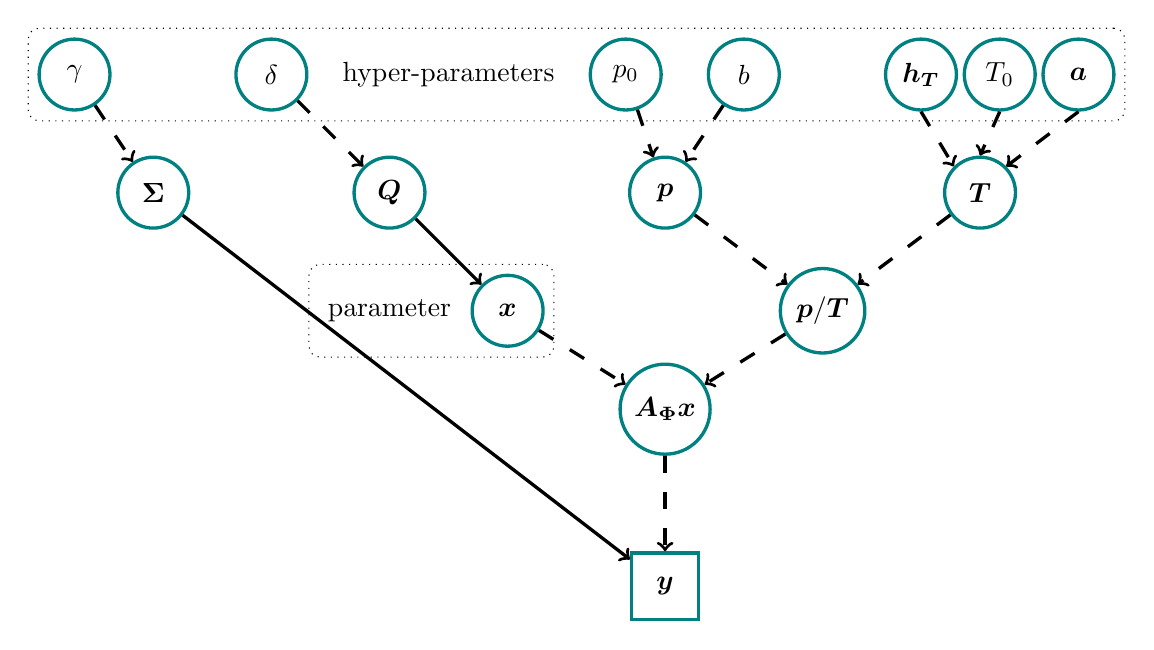
\begin{tikzpicture}
		\node[roundnode2] at (-4.5,6.5) (Q)     {$\bm{Q}$};
		\node[roundnode2] at (-3,5) (x)     {$\bm{x}$};
		%\node[roundnode2] at (-1,3.75) (A)    {$\bm{A}_{\bm{\Phi}} \coloneqq \bm{M}\bm{A}_L(p_0,b,T_0,\bm{h_T},\bm{a})$};
			\node[roundnode2] at (-1,3.75) (A)    {$\bm{A}_{\bm{\Phi}} \bm{x}$};
		%\node[roundnode2] at (-1,2.5) (u)    {$\Omega$};
		\node[rectnode] at (-1,1.5) (y)    {$\bm{y}$};
		%\node[roundnode2] at (-3,2.5) (e)    {$\bm{\eta}$};
		\node[roundnode2] at (-7.5,6.5) (S)    {$\bm{\Sigma}$};
		\node[roundnode2] at (-8.5,8) (s)    {$\gamma$};
		\node[roundnode2] at (-6,8) (d)    {$\delta$};
		\node[roundnode2] at (3,6.5) (t)     {$\bm{T}$};
		\node[roundnode2] at (-1,6.5) (p)     {$\bm{p}$};
		\node[roundnode2] at (1,5) (pt)     {$\bm{p}/\bm{T}$};
		\node[roundnode2] at (0,8) (b1)    {$b$};
		%\node[roundnode2] at (1,8) (b2)    {$b_2$};
		%\node[roundnode2] at (-2,8) (h1)    {$h_{0}$};
		\node[roundnode2] at (-1.5,8) (p0)    {$p_0$};
		\node[roundnode2] at (2.25,8) (ht)    {$\bm{h_T}$};
		\node[roundnode2] at (3.25,8) (ct)    {$T_0$};
		\node[roundnode2] at (4.25,8) (at)    {$\bm{a}$};
		
		%\node[roundnode2] at (0,10) (b1hyp)    {$\bm{\theta}_{b}$};
		%\node[roundnode2] at (-2.5,10) (h1hyp)    {$\bm{\theta}_{h_{0}}$};
		%\node[roundnode2] at (-1.5,10) (p0hyp)    {$\bm{\theta}_{p_{0}}$};
		%\node[roundnode2] at (2,10) (hthyp)    {$\bm{\theta}_{\bm{h}_T}$};
		%\node[roundnode2] at (3.25,10) (cthyp)    {$\bm{\theta}_{T_{0}}$};
		%\node[roundnode2] at (4.5,10) (athyp)    {$\bm{\theta}_{\bm{a}}$};
		
		%\node[roundnode2] at (-8.5,10) (shyp)    {$\bm{\theta}_{\gamma}$};
		%\node[roundnode2] at (-6,10) (dhyp)    {$\bm{\theta}_{\delta}$};
		
		%Lines
		
		
		\draw[->, very thick] (S) -- (y);
		\draw[->, mydotted, very thick] (s) -- (S);
		%\draw[->, very thick] (u) -- (y);
		\draw[->, mydotted, very thick] (A) -- (y);
		\draw[->, mydotted,  very thick] (x) -- (A);
		\draw[->, mydotted, very thick] (p) -- (pt);
		\draw[->, mydotted, very thick] (t) -- (pt);
		\draw[->, mydotted, very thick] (pt) -- (A);
		%\draw[->, mydotted, very thick] (h1) -- (p);
		\draw[->, mydotted, very thick] (p0) -- (p);
		\draw[->, mydotted, very thick] (b1) -- (p); 
		%\draw[->, very thick] (b2.south) -- (p.east); 
		\draw[->, mydotted, very thick] (d) -- (Q); 
		%\draw[->, mydotted, very thick] (e) -- (y); 
		
		\draw[->, very thick] (Q.south east) -- (x.north west); 
		\draw[->, mydotted, very thick] (ht.south) -- (t.north west);
		\draw[->, mydotted, very thick] (ct.south) -- (t.north);
		\draw[->, mydotted, very thick] (at.south) -- (t.north east);
		
		
		%\draw[->, very thick] (b1hyp) -- (b1);
		%\draw[->, very thick] (h1hyp) -- (h1);
		%\draw[->, very thick] (p0hyp) -- (p0);
		%\draw[->, very thick] (hthyp) -- (ht);
		%\draw[->, very thick] (cthyp) -- (ct);
		%\draw[->, very thick] (athyp) -- (at);
		%\draw[->, very thick] (shyp) -- (s);
		%\draw[->, very thick] (dhyp) -- (d);
		
		\node[fit=(s)(at),draw,dotted,black, rounded corners] {};
		\node[align =center] at (-3.75,8) (T1) {hyper-parameters};
		\node[align =center] at (-4.5,5) (T2) {parameter};
		\node[fit=(x)(T2),draw,dotted,black, rounded corners] {};
		
	\end{tikzpicture} 
	\caption[Directed acyclic graph of Bayesian model for ozone $\bm{x}$, pressure $\bm{p}$ and temperature $\bm{T}$.]{DAG of the hierarchical Bayesian model including ozone $\bm{x}$, pressure $\bm{p}$ and temperature $\bm{T}$. The hyper-parameters $\bm{h}_T= \{ h_{T,1}, h_{T,2},h_{T,3},h_{T,4},h_{T,5},h_{T,6}\}$, $\bm{a} = \{ a_0, a_1, a_2,a_3,a_4,a_5,a_6\}$, $T_0$, $b$ and $p_0$ deterministically (dotted line) describe pressure through Eq.~\ref{eq:pressFunc} and temperature through Eq.~\ref{eq:tempFunc}. The hyper-prior distributions $\pi(p_0,b,T_0,\bm{h_T},\bm{a})$ are a normal distributions, see Eq.~\ref{eq:aPrior} to Eq.~\ref{eq:lastprior}. 
		%That is why $\bm{\theta}_{\bm{h}_T},\bm{\theta}_{\bm{a}}, \bm{\theta}_{T_{0}},\bm{\theta}_{b} , \bm{\theta}_{p_0}$ represent means and STDs e.g.,~$b \sim \mathcal{N}(\mu_b, \sigma^2_b)$ and $\bm{\theta}_{b} = \{\mu_b, \sigma_b\}$.
		The hyper-prior distributions $\pi(\gamma)$ and $\pi(\delta)$ are gamma distributions, see Eq.~\ref{eq:priorDelFull} and Eq.~\ref{eq:priorGamFull}.
		The ozone parameter $\bm{x}$ is statistically (solid line) described by the prior distribution $\bm{x}| \delta \sim \mathcal{N}(0,(\delta \bm{L})^{-1}) $. 
		Here, the hyper-parameter $\delta$ accounts for smoothness in the ozone profile and defines the precision matrix $\bm{Q} = \delta \bm{L}$ as in Eq.~\ref{eq:GLapl}.
		The approximated forward model $\bm{A}_{\bm{\Phi}} \coloneqq \bm{M}\bm{A}_L(p_0,b,T_0,\bm{h_T},\bm{a})$ with $\bm{\Phi}  \coloneqq \{p_0, b, T_0,\bm{h}_T,\bm{a} \}$ describes the noise-free data $\bm{A}_{\bm{\Phi}} \bm{x}$.
		An observed (square box) data set $\bm{y}$ includes some additive random noise described by the noise covariance $\bm{\Sigma} = \gamma^{-1} \bm{I}$.}
	%Given the data we like to determine the marginal posterior distribution over the hyper-parameters $\pi(\bm{\theta}, \delta, \gamma | \bm{y})$ first and then the conditional posterior distribution for ozone $\pi(\bm{x}|\bm{\theta}, \delta, \gamma, \bm{y})$, utilising the MTC scheme.}
\label{fig:DAGComplete}
\end{figure}
The DAG in Fig.~\ref{fig:DAGComplete} visualises the measurement process and conditional dependencies between the parameter $\bm{x}$ and the hyper-parameters $\bm{\theta} = \{p_0,b,T_0,\bm{h_T},\bm{a}, \delta , \gamma\}$.
This hierarchical Bayesian framework includes the hyper-parameters $p_0, b$ for the pressure profile (see Eq.~\ref{eq:pressFunc}), $\bm{a}, \bm{h}_T, T_0$ for the temperature profile (see Eq.~\ref{eq:tempFunc}), $\delta$ for the ozone smoothness and $\gamma$ for the noise precision.
The hyper-parameters are described by the hyper-prior distribution $\pi(p_0,b,T_0,\bm{h_T},\bm{a}, \delta,\gamma)$ (see Sec.~\ref{subsec:PriorFull}).
Through their respective prior distributions, pressure $\bm{p}$, temperature $\bm{T}$ and ozone $\bm{x}$ progress deterministically (dashed line) into the forward model via $\bm{x} \times \bm{p} / \bm{T}$ and generate a space of all possible noise-free data $\Omega$.
Note that other variables in the RTE, such as the internal partition function and the black body radiation, are dependent on temperature as well (see Eq.~\ref{eq:RTE}).
Finally, we observe (square box) some data $\bm{y}$ with additive normally distributed noise with zero mean and covariance $\bm{\Sigma} = \gamma^{-1} \bm{I}$.
For brevity, we define the forward model matrix as
\begin{align}
\bm{A}_{\bm{\Phi}} \coloneqq \bm{M}\bm{A}_L(p_0,b,T_0,\bm{h_T},\bm{a}) 
\end{align}
with $\bm{\Phi}  \coloneqq \{p_0,b,T_0,\bm{h_T},\bm{a}  \}$ accounting for the all pressure and temperature related hyper-parameters and $\bm{M}$ is an affine approximation.
If $\bm{M} =\bm{I}$, then the forward model is based on the linearised RTE and the absorption term in the RTE, see Eq.~\ref{eq:absRTE}, is neglected
%First $\bm{M} = \bm{I}$ is set to the identity matrix and the problem is treated as a linear inverse problem where the non-linear term in the RTE is neglected.
%Once an affine approximation of the non-linear RTE is obtained using results based on the linearised RTE, the non-linear RTE is approximated as $\bm{A}(\bm{p},\bm{T},\bm{x}) \approx \bm{A}_{\bm{\Phi}} \bm{x}$, where $\bm{M}$ is an affine map.


The distributions of the hierarchical Bayesian framework are:
\begin{subequations}
\label{eq:BayMode}
\begin{align}
	\bm{y} |  \bm{x},\bm{\Phi},\delta,\gamma  &\sim \mathcal{N}(\bm{A}_{\bm{\Phi}}  \bm{x}, \gamma^{-1} \bm{I}) \label{eq:likelihoodFull} \\
	\bm{x}| \delta  &\sim \mathcal{N}(\bm{0}, (\delta \bm{L})^{-1} ) \label{eq:priorXFull} \\
	\delta  &\sim \mathcal{T}(\alpha_{\delta} , \beta_{\delta} )\label{eq:priorDelFull} \\
	\gamma  &\sim \mathcal{T}(\alpha_{\gamma}, \beta_{\gamma})\label{eq:priorGamFull} \\
	\bm{a}  &\sim \mathcal{N}(\bm{\mu}_{\bm{a}}, \bm{\Sigma}_{\bm{a}})\label{eq:aPrior}\\
	\bm{h}_{\bm{T}}  &\sim \mathcal{N}(\bm{\mu}_{T}, \bm{\Sigma}_{\bm{h}_T}) \\
	T_0  &\sim \mathcal{N}(\mu_{T_0}, \sigma^2_{T_0} )\\
	p_0  &\sim \mathcal{N}(\mu_{p_0}, \sigma^2_{p_0} )\\
	b  &\sim \mathcal{N}(\mu_b, \sigma^2_b )  \label{eq:lastprior}  \, .
\end{align}
\end{subequations}
Due to Gaussian noise $\pi(\bm{y} |  \bm{x},\bm{\Phi},\delta,\gamma )$ is a normally distributed likelihood function and Eq.~\ref{eq:priorXFull} to Eq.~\ref{eq:lastprior} denote prior distributions.
The hyper-prior scales, shapes, means and variances are explicitly given in Tab.~\ref{tab:priors}.
%Before formulating the posterior distribution, we carefully define $\bm{\theta}_{\gamma}, \bm{\theta}_{\delta},\bm{\theta}_{p_0},\bm{\theta}_{b},\bm{\theta}_{\bm{h}},\bm{\theta}_{T_0},\bm{\theta}_{\bm{a}}$, the hyper-prior scales, shapes, means and variances, which are explicitly given in Tab.~\ref{tab:priors}.
\begin{table}[ht!]
	\centering
	\begin{tabular}{ |c||c|c|c|c|  }
		\hline
		& &\multicolumn{2}{|c|}{TT bounds}& \\
		\hline
		model parameters& priors&\makecell{lower}& \makecell{upper\\
		}&Context\\
		\hhline{|=||=|=|=|=|}
		$\bm{x}$ &$\mathcal{N}(0,(\delta \bm{L})^{-1})$ & - &-& $\bm{x}$\\ \hline
		$\delta$ &$\mathcal{T}(1,10^{-35})$ & $5\times 10^{10}$&$1 \times 10^{13}$& $\bm{x}$\\ \hline
		$\gamma$ & $\mathcal{T}(1,10^{-35})$ &$8\times10^{14}$ &$6\times10^{15}$& $\bm{y}$\\ \hline
		$b$ &  $\mathcal{N}(0.174,(0.01)^2)$& 0.129& 0.214 &$\bm{p}$\\ \hline
		$h_{T,1}$ &  $\mathcal{N}(11,(1.5)^2)$&5.4 &16.3&$\bm{T}$\\ \hline
		$T_{0}$ &  $\mathcal{N}(288.15,(10)^2)$& 247 &326&$\bm{T}$\\ \hline
		$p_0$ &  $\mathcal{N}(1311,(20)^2)$&1237 &1387&$\bm{p}$\\ \hline
		$h_{T,3}$ &  $\mathcal{N}(32.3,(2.5)^2)$&22.9&41.7&$\bm{T}$\\ \hline
		$a_{1}$ &  $\mathcal{N}(0,(0.1)^2)$&-0.38 &0.38&$\bm{T}$\\ \hline
		$h_{T,2}$ &  $\mathcal{N}(20.1,(0.7)^2)$&17.2 &22.7&$\bm{T}$\\ \hline
		$a_{0}$ &  $\mathcal{N}(-6.5,(0.01)^2)$&-6.54 &-6.47&$\bm{T}$\\ \hline
		$a_{2}$ &  $\mathcal{N}(1,(0.01)^2)$&0.97 &1.03&$\bm{T}$\\ \hline
		$a_{3}$ &  $\mathcal{N}(2.8,(0.1)^2)$&2.5 &3.1&$\bm{T}$\\ \hline
		$h_{T,4}$ &  $\mathcal{N}(47.4,(0.5)^2)$&45.5 &49.3&$\bm{T}$\\ \hline
		$a_{4}$ &  $\mathcal{N}(0,(0.1)^2)$&-0.38 &0.38&$\bm{T}$\\ \hline
		$h_{T,5}$ &  $\mathcal{N}(51.4,(0.5)^2)$&49.5 &53.3&$\bm{T}$\\ \hline
		$a_{5}$ &  $\mathcal{N}(-2.8,(0.1)^2)$&-3.18 &-2.43&$\bm{T}$\\ \hline
		$h_{T,6}$ &  $\mathcal{N}(71.8,(3)^2)$&60.5 &83.1&$\bm{T}$\\ \hline
		$a_{6}$ & $\mathcal{N}(-2,(0.01)^2)$ &-2.04 &-1.96&$\bm{T}$\\
		\hline
	\end{tabular}
	\caption[Summary of relevant parameter characteristics, bounds and sampling statistics.]{Summary of relevant parameter and hyper-parameters bounds and statistics, ordered as in the TT format according to their correlation structure. We denote $\mathcal{N}(\mu= \text{mean},\sigma^2= \text{variance})$ as the Gaussian and $\mathcal{T}(\alpha = \text{scale}, \beta = \text{rate})$ as the Gamma distribution.}
	\label{tab:priors}
\end{table}
\clearpage


%Note that we fit one exponential function to ground truth pressure values between $h_{L,0} \approx 7$km and $h_{L,n} \approx 82$, so that the pressure value $p_0$ may be different to true sea-level pressure values at $h = 0$km due to that approximation.
\subsection{Posterior Distribution}
\label{sec:PostDistr}
As explained in Sec.~\ref{subsec:TheoMTC}, we factorise the posterior
\begin{align}
	\pi( \bm{x},\bm{\Phi}, \delta, \gamma| \bm{y}) \propto \pi(\bm{y}| \bm{x},\bm{\Phi},\delta,\gamma) \pi( \bm{x},  \bm{\Phi},\delta,\gamma)
\end{align}
into 
\begin{align}
	\pi( \bm{x}, \bm{\Phi}, \delta,\gamma| \bm{y}) =\pi( \bm{x}| \bm{\Phi},\delta,\gamma, \bm{y})\pi( \bm{\Phi},\delta,\gamma | \bm{y})
\end{align}
the marginal posterior $\pi(\bm{\Phi},\delta ,\gamma| \bm{y})$ and full conditional posterior $\pi( \bm{x}| \bm{\Phi},\delta,\gamma, \bm{y})$ (see Eq.~\ref{eq:MTC}).
%Fox and Norton call this method the marginal and then conditional method (MTC) \cite{fox2016fast}, where we break the correlation structure between $\bm{x}$ and $\gamma, \delta$ as illustrated in Fig. \ref{fig:RueHeld} by marginalising over $\bm{x}$.
As discussed in~\cite{fox2016fast}, for the linear-Gaussian case, $\bm{x}$ cancels in the marginal posterior over the hyper-parameters.
Following the MTC scheme, we characterise the marginal posterior over the hyper-parameters $\bm{\theta} = \{ \bm{\Phi}, \gamma, \delta \}$ first and then draw samples from the full conditional posterior for the parameter $\bm{x}$.

%Here, the marginal posterior distribution $\pi(\bm{\theta}| \bm{y})$ over the hyper-parameters $\bm{\theta} = \{ \bm{\Phi}, \gamma, \delta \}$ and the full conditional posterior distribution  $\pi(\bm{x}|\bm{\theta},\bm{y})$ for the parameter $\bm{x}$ are formulated.
%To draw samples from the marginal posterior $\pi(\bm{\theta}| \bm{y})$ we utilise a TT approximation on a predefined grid to generate samples via the SIRT method with an MH correction step.
%In doing so, the reader is guided through the process of obtaining an efficient higher-dimensional TT approximation.
%Lastly, the RTO method is utilised to draw ozone samples from the full conditional posterior $\pi(\bm{x}|p_0,b,T_0,\bm{h_T},\bm{a} ,\delta, \gamma, \bm{y})$.
%Recall that $\bm{x} \in \mathbb{R}^n$ with $n = 34$ and $\bm{y} \in \mathbb{R}^m$ with $m = 30$, and that the linear forward model matrix $\bm{A}_{\bm{\Phi}}$ is depending on the hyper-parameter defined as $\bm{\Phi}  \coloneqq \{p_0,b,T_0,\bm{h_T},\bm{a}  \}$.
%Consequently, the marginal posterior is denoted as $\pi( \bm{\Phi},\delta,\gamma  | \bm{y}) $ and the full conditional posterior as $\pi(\bm{x}|\bm{\Phi}, \delta, \gamma, \bm{y})$.

\subsubsection{Marginal Posterior -- Pressure and Temperature}
As in~\cite{fox2016fast}, the marginal posterior is given as
\begin{align}
\pi( \bm{\Phi},\delta,\gamma  | \bm{y}) \propto &  \delta^{n/2} \gamma^{m/2}   \exp{ \Bigl\{ - \frac{1}{2} g ( \bm{\Phi},\delta,\gamma ) - \frac{\gamma}{2} f (\bm{\Phi},\delta,\gamma ) \Bigr\}} \pi(\bm{\Phi},\delta,\gamma ) \, ,
\label{eq:MargPostFull}
\end{align}
with,
\begin{subequations}
\label{eq:fandgTrue}
\begin{align}
	&f ( \bm{\Phi},\delta, \gamma) = \bm{y}^T \bm{y} - \big(\bm{A}_{\bm{\Phi}}^T \bm{y}\big)^T \big(\gamma \bm{A}_{\bm{\Phi}}^T  \bm{A}_{\bm{\Phi}} + \delta \bm{L}\big)^{-1} \big(\bm{A}_{\bm{\theta}}^T \bm{y}\big)  \label{eq:fFullAppl} \, ,  \\
	&\text{and } g(\bm{\Phi},\delta, \gamma) = \log \det \big(\gamma \bm{A}_{\bm{\Phi}}^T  \bm{A}_{\bm{\Phi}} + \delta \bm{L}\big) \label{eq:gFullAppl} \, .
\end{align}
\end{subequations}
For each evaluation of $\pi( \bm{\Phi},\delta,\gamma  | \bm{y})$, $\bm{A}_{\bm{\Phi}}$ is composed as in Section~\ref{ch:formodel}, and $f$ and $g$ are calculated directly using the Cholesky decomposition via the Python functions \texttt{torch.linalg.cholesky} and \texttt{torch.cholesky\_solve}.


\subsubsection{Full Conditional Posterior -- Ozone}
\label{subsec:firstCond}
As in~\cite{SIMPSON201216}, consider the joint Gaussian distribution
\begin{align}
	\begin{pmatrix}
		\bm{x} \\
		\bm{y}
	\end{pmatrix}\sim \mathcal{N}\left[  \begin{pmatrix}
		\bm{\mu} \\
		\bm{A}\bm{\mu}
	\end{pmatrix},\begin{pmatrix}
		\bm{Q} + \bm{A}_{\bm{\Phi}}^T \bm{\Sigma}^{-1} \bm{A}_{\bm{\Phi}} & - \bm{A}_{\bm{\Phi}}^T \bm{\Sigma}^{-1} \\
		\bm{\Sigma}^{-1} \bm{A}_{\bm{\Phi}} & \bm{\Sigma}^{-1} 
	\end{pmatrix}^{-1} \right] \, 	\label{eq:jointMultiGaus}
\end{align}
with $\bm{\Sigma}^{-1} = \gamma \bm{I} $ and $\bm{Q}  = \delta \bm{L} $ and $\bm{\mu} = \bm{0}$.
Then the full conditional posterior distribution of ozone 
\begin{align}
	\bm{x}|\bm{\Phi}, \delta, \gamma, \bm{y}  \sim \mathcal{N}\big(  (\bm{A}_{\bm{\Phi}}^T \bm{A} + \delta / \gamma \bm{L} )^{-1} \bm{A}_{\bm{\Phi}}^T \bm{y}, (  \gamma \bm{A}_{\bm{\Phi}}^T \bm{A}_{\bm{\Phi}} + \delta \bm{L}  \big) \, \label{eq:CondPost},
\end{align}
is a normal distribution and samples can be drawn via the randomise-then-optimise (RTO) method, see Sec.~\ref{subsec:FullCondPost} and~\cite{bardsley2012mcmc, bardsley2014randomize,BardsleyTC2019RTO,fox2016fast}.


\section{Results}
In this section, the results are presented.
Some data is simulated as described in Sec.~\ref{sec:SimDat} and plotted in Fig.~\ref{fig:Data}.
Given the data the inverse problem is treated as a linear inverse problem by neglecting the non-linear absorption in the RTE.
With the simulated data and the previously defined priors, the marginal and full conditional posterior are well defined and the MTC scheme is applied.
The marginal posterior is approximated by a tensor-train (TT) and the squared inverse Rosenblatt transform (SIRT)~\cite{cui2022deep} is employed to generate samples from the marginal posterior.
Conditioned on those hyper-parameter samples the randomise-then-optimise (RTO) method is used to sample from the full conditional posterior.
Then an affine approximation is calculated and the non-linear forward model is approximated by the affine map and the linear forward model.
With the approximated forward model the just-explained methodology (TT approximation and RTO) is repeated.
Finally, we present posterior ozone, pressure and temperature profiles based on the approximated forward model.

\begin{figure}[ht!]
	\centering
	\includegraphics[]{TTPapData.png}
	\caption[]{Non-linear noise-free data and non-linear noisy data at different tangent heights. Negative noisy data values are not shown due to logarithmic scaling.}
	\label{fig:Data}
\end{figure} 
\clearpage
\subsection{Linear Forward Model}
\label{subsec:ResLinForMod}
As already mentioned the forward model is defined as:
\begin{align}
	\bm{A}_{\bm{\Phi}} \coloneqq \bm{M} \bm{A}_L(\bm{\Phi}) \, 
\end{align}
with $\bm{\Phi} = \{p_0,b,T_0,\bm{h_T},\bm{a}\}$ and $\bm{M} = \bm{I}$, for now.


\subsubsection{Tensor-Train Approximation of the Marginal Posterior}
Instead of using conventional Markov-Chain Monte-Carlo methods, such as e.g., the t-walk~\cite{christentwalkaccess}, to generate samples from the marginal posterior, the marginal posterior is approximated directly using a TT representation.
In the following a brief introduction to the TT format is provided.
For more technical details we refer the reader to~\cite{dolgov2020approximation} for the inverse Rosenblatt transform (IRT), to~\cite{cui2022deep} for the SIRT and to~\cite{OSELEDETS2010TTCross} for the TT-cross algorithm that generates a function approximation in the TT format.



\paragraph{Background on Tensor-Train Approximation}
Assume the target function is $\pi( \bm{\Phi},\delta,\gamma  | \bm{y})$ and the input $\bm{\theta} \coloneqq \{\bm{\Phi},\delta,\gamma  \} \in \mathbb{R}^d  $ is $d$-dimensional.
First, a $d$-dimensional grid with $n$ grid points in each dimension the parameter space is defined.
Usually, representing the marginal posterior naively as a $d$-dimensional tensor with $n^d$ grid points is computationally not feasible. 
Instead a TT can be employed to approximate the target function on that parameter space with far fewer function evaluations.
In practice, a TT approximation may have negative or zero values in regions where the true function value is small and positive.
That is why, to ensure non-negativity, we approximate the square root of $\pi( \bm{\theta}  | \bm{y})$ over the whole parameter space, which can be written as:
\begin{align}
	\sqrt{\pi( \bm{\theta}  | \bm{y})} \approx \tilde{g}(\bm{\theta}) =  \bm{G}_1(\theta_1), \dots, \bm{G}_k(\theta_k), \dots, \bm{G}_d(\theta_d)\, ,
\end{align}
where each $\bm{G}_k \in \mathbb{R}^{r_{k-1}\times n \times r_{k}}$ is a TT core.
Further, $r_{k}$ are the ranks of the individual cores and bounded by $r_{0} = 1$ and $r_{d} = 1$.
For now, assume the ranks $r_k = r$ for $k =1, \dots, d-1$, then the TT approximates the function space with $n \times r^2 \times (d-2) + n \times r \times 2$ instead of the $n^d$ function evaluations.

Given a TT approximation, samples from the target function are generated via the IRT scheme~\cite{dolgov2020approximation}, more precisely, the SIRT as ~\cite{cui2022deep} since we approximate the square root of the target function.
Within this scheme a sequence of 1-dimensional functions can be constructed, so that
\begin{align}
	\label{eq:IRTcondMarg}
	\begin{split}
		\pi( \bm{\theta}  | \bm{y}) =&  \quad \pi(\theta_1 | \bm{y}) \\
		& \quad \times \pi( \theta_2 | \theta_1, \bm{y}) \\
		&\quad \times\pi( \theta_3 | \theta_2,\theta_1, \bm{y})  \\
		&\quad \times\pi( \theta_4 | \theta_3, \theta_2,\theta_1, \bm{y}) \\
		& \quad \quad \vdots \\
		&\quad \times \pi( \theta_d | \theta_{d-1}, \dots, \theta_4,\theta_3, \theta_2,\theta_1, \bm{y}) \, .
	\end{split}
\end{align}
We call each function $\pi( \theta_k | \theta_{k-1},\dots, \theta_1, \bm{y})$ the 'conditional marginal' because it is conditioned on $\theta_{k-1},\dots, \theta_1, $ and marginalised over $\theta_{k+1} , \dots, \theta_d$.
To obtain these is computationally relatively cheap because each of the TT cores is representative for one dimension in the parameter space and hence it is easy to integrate over the individual parameters $\theta_k \in \bm{\theta}$ for $k = 1, \dots, d$.
The marginal distribution of the first dimension is computed as:
\begin{align}
	\begin{split}
		\pi(\theta_1 | \bm{y}) \approx \frac{1}{z}  \bm{G}_1^2(\theta_1)  
		\int \bm{G}_{2}^2(\theta_{2}) \, \diff \theta_{2}\cdots 
		\int \bm{G}_d^2(\theta_d)  \, \diff \theta_d ,
	\end{split}
\end{align}
where each of the integrals reduce a core $\bm{G}_k \in \mathbb{R}^{r_{k-1}\times n \times r_{k}}$ to $\int \bm{G}_k^2(\theta_k)  \, \diff \theta_k \in \mathbb{R}^{r_{k-1} \times r_{k}}$ and $z$ is a normalisation constant, see~\cite{cui2022deep} for more details.
If you want to use a quadrature scheme to calculate expectations, e.g., $\mathbb{E}_{	\pi( \bm{\theta}  | \bm{y})} [f(\bm{\theta})]$, or are only interested in the individual marginals you are done here since other marginals can be computed the same way.
Note that, for a specific parameter value $\theta_k$ the core $\bm{G}^2_k(\theta_k)\in \mathbb{R}^{r_{k-1} \times r_{k}}$ is given according to the used interpolation basis, see, e.g.,~\cite{dolgov2020approximation}, for piecewise linear interpolation (first order Lagrange polynomial).

The 'conditional marginal' defines a mapping from the uniform distribution to the target function, which is constructed via the cumulative distribution function (CDF)
\begin{align}
	F(\theta_k) = \int_{-\infty}^{\theta_k} \pi( \hat{\theta}_k | \theta_{k-1},\dots, \theta_1, \bm{y}) \diff \hat{\theta}_k  \, .
	\label{eq:CurrCDF}
\end{align}
Then a uniformly distributed random variable $\bm{u} \sim \mathcal{U} [0,1]^d$ is projected onto the parameter space via the inverse
\begin{align*}
	\theta_k = F^{-1}(u_k)
\end{align*}
with $u_k \in \bm{u}$.
This scheme is repeated for each 'conditional marginal' in Eq.~\ref{eq:IRTcondMarg} until a sample $\bm{\theta} \sim \tilde{\pi} (\bm{\theta}|\bm{y})$ is obtained.

Since the samples $\{ \bm{\theta}^{(1)} , \dots, \bm{\theta}^{(N)}\} \sim \tilde{\pi} (\bm{\theta}|\bm{y})$ are drawn from an approximation they are corrected with an Metropolis--Hastings (MH) algorithm~\cite{dolgov2020approximation}.
To take one MH correction step from a current state $\bm{\theta}$ to a proposed state $\bm{\theta}^{\prime} $ the ratio
\begin{align}
	h(\bm{\theta}, \bm{\theta}^{\prime}  ) = \frac{\pi( \bm{\theta}^{\prime}  | \bm{y}) \tilde{\pi}( \bm{\theta}  | \bm{y})}{\pi( \bm{\theta}  | \bm{y}) \tilde{\pi}( \bm{\theta}^{\prime}   | \bm{y})}
\end{align}
is computed and the proposal $ \bm{\theta}^{\prime}$ is accepted with probability
\begin{align}
	\alpha(\bm{\theta}, \bm{\theta}^{\prime}  )  = \min (h(\bm{\theta}, \bm{\theta}^{\prime}  ) ,1) \, .
\end{align}
If $ \bm{\theta}^{\prime}$ is accepted the next current state is $ \bm{\theta}= \bm{\theta}^{\prime}$, if $ \bm{\theta}^{\prime}$ is rejected $ \bm{\theta}$ remains the current state.


In practice, a small constant $\xi$ according to the L2-norm error of the TT approximation is added so that 
\begin{align}
	\pi( \bm{\theta}  | \bm{y}) \approx \tilde{\pi}( \bm{\theta}  | \bm{y}) = \frac{1}{z} (\xi + \tilde{g}(\bm{\theta})^2) \, .
\end{align}
This has the consequence that the chain of the MH correction algorithm is uniformly geometrically convergent (and ergodic~\cite{dolgov2020approximation}) towards $\pi( \bm{\theta}  | \bm{y})$, because
\begin{align}
	\label{eq:ErroRatio}%\tilde{w} =
	\left\lVert	\frac{\pi( \bm{\theta}  | \bm{y})}{\tilde{\pi}( \bm{\theta}  | \bm{y})} \right\rVert_{\infty} = \sup \frac{\pi( \bm{\theta}  | \bm{y})}{\xi + \tilde{g}(\bm{\theta})^2} < \infty
\end{align}
is bounded~\cite{cui2022deep}.
Without $\xi$ the TT approximation $\tilde{g}(\bm{\theta})^2$ may be arbitrarily small in regions where the true function is small and the ratio in Eq.~\ref{eq:ErroRatio} can not be bounded.
With $\xi$ we introduce a more or less uniform error.
In~\cite{cui2022deep} it is shown that, if $\xi$ is chosen according to the L2-norm error
\begin{align}
	\left\lVert \tilde{g}(\bm{\theta}) - \sqrt{\pi( \bm{\theta}  | \bm{y})}\right\rVert_2\leq \epsilon \, ,
\end{align}
then the approximation satisfies the error bound
\begin{align}
	\left\lVert \sqrt{\tilde{\pi}( \bm{\theta}  | \bm{y})}- \sqrt{\pi( \bm{\theta}  | \bm{y})}\right\rVert_2 \leq \sqrt{2} \epsilon \, .
\end{align}


In theory, the SIRT scheme provides independent samples, but in practice, every system produces correlated samples.
To assess this correlation, we calculate the integrated autocorrelation time (IACT) as in~\cite{wolff2004monte,wolff2002LecNot} using the Python implementation from~\cite{drikHesse}.
Note that we define the IACT
\begin{align}
	\tau_{\text{int}}  \coloneqq  \Bigg(  1 + 2 \sum_{t = 1}^{W} \frac{\Gamma(t)}{\Gamma(0)}  \Bigg)  
\end{align} 
as in~\cite{fox2016fast} with an autocorrelation coefficient $\Gamma(t)$.
This is twice the value of the IACT in~\cite[pp. 103-105]{wolff2002LecNot} and~\cite{wolff2004monte,drikHesse}, as commonly defined within the physics community.
U. Wolff~\cite{wolff2004monte} (and the Python implementation by D. Hesse~\cite{drikHesse}) provide a way to not only calculate the IACT safely (choosing the summation window $W$) but also to quantify the errors of the estimated IACT.
%The IACTs are $\tau_{\text{int},\lambda} = 1.05\pm0.04$ and $\tau_{\text{int},\gamma} =0.99\pm0.03$ based on a chain with 10000 samples.
%So every second sample via the IRT scheme presents an independent marginal posterior sample.
%Conditioned on an independent sample from the marginal posterior, one can draw an independent sample from the full conditional posterior.
%Further we can use that to bound the maximum absolute error $\epsilon$ as in.
%\begin{align}
%	\frac{\tau_{\text{int}} -1 }{2}	 \leq \tilde{w} - 1
%\end{align}
%We can use 
%\begin{align}
%	\tau_{\text{int}} -1 
%\end{align}
%as an error estimate.

\clearpage
\paragraph{Generate and use Tensor-Train Approximation}
To generate a TT approximation for $\pi( \bm{\theta}  | \bm{y})$ we use the \texttt{deep-tensor-py} package~\cite{alexDeepPy}, which implements the TT-cross algorithm~\cite{OSELEDETS2010TTCross}.
Further, A. de Beer~\cite{alexDeepPy} has implemented the SIRT scheme from~\cite{cui2022deep}.
By exploratory analysis we define ranks \textcolor{red}{$r=[10,10,\dots,2]$} manually and set the grid size $n=30$ for the 18-dimensional parameter space, see Tab.\ref{tab:priors} for the grid bounds.
Then one sweep (left-to-right and right-to-left) by the TT-cross with first order Legendre polynomials as basis functions provides an accurate enough function approximation of the marginal posterior.
This requires \textcolor{red}{$xxxx$} function evaluations.
Note that we arranged the hyper-parameter space so that highly correlated hyper-parameters are adjacent, see red boxes in Fig.~\ref{fig:CorrPlot}.
The Python code \textcolor{red}{will be}/is available here: \url{https://deeptransport.github.io/deep-tensor-py/examples/}.
To generate a TT approximation and $\approx 2000$ samples, see Fig.~\ref{fig:CorrPlot}, from the marginal posterior including the MH-correction step takes $\approx 1$min on a basic laptop.
The maximum IACT is $1.2 \pm 0.1$, so every second sample via the SIRT-MH scheme is an independent sample from the marginal posterior.
Conditioned on an independent marginal posterior sample $\bm{\theta}^{(k)} \sim \pi(\bm{\theta}| \bm{y})$ the RTO method can be used to generate a full conditional posterior sample $\bm{x}^{(k)} \sim \pi(\bm{x}|\bm{\theta}^{(k)}, \bm{y})$.  
\clearpage
\begin{figure}[h!]% will be the left-side figure
	\includegraphics[]{1stCorrPlot.png}
	\caption[Correlation plot of samples from TT approximation]{Plot of 1000 independent samples from the marginal posterior $\pi(\bm{\Phi},\delta,\gamma|\bm{y})$ based on the linearised forward model via the SIRT-MH scheme. We plot the Pearson correlation coefficient ranging from $-1$ to $1$ for each hyper-parameter pair.}
	\label{fig:CorrPlot}
\end{figure}
\begin{figure}% will be the right-side figure
	\includegraphics[]{2ndCorrPlot.png}
	\caption*{Correlation plot of samples from the marginal posterior $\pi(\bm{\Phi},\delta,\gamma|\bm{y})$ based on the linearised forward model via the SIRT-MH scheme.}
\end{figure}
\clearpage
\subsubsection{Samples from the Full Conditional Posterior}
\label{subsec:FullCondPost}

To sample an posterior ozone profile from the full conditional $\pi(\bm{x} |\bm{\theta}, \bm{y})$ with $\bm{\theta} = \{\bm{\Phi},\delta, \gamma\}$ we use the RTO method, as in~\cite{bardsley2012mcmc, bardsley2014randomize,BardsleyTC2019RTO,fox2016fast}.
To derive the RTO method, rewrite the full conditional posterior as
\begin{align}
	\pi(\bm{x} | \bm{\Phi}, \delta, \gamma, \bm{y}) & \propto \pi(\bm{y}|\bm{x}, \bm{\Phi}, \gamma) \pi(\bm{x}| \delta)\\
	&\propto \exp \left(-\frac{1}{2} (\bm{A}_{\bm{\Phi}} \bm{x} - \bm{y})^T \bm{\Sigma}^{-1} (\bm{A}_{\bm{\Phi}}  \bm{x} - \bm{y})\right) \exp \left(-\frac{1}{2} (\bm{\mu} - \bm{x} )^T \bm{Q}(\bm{\mu} - \bm{x} ) \right),\\
	& = \exp \left( - \frac{1}{2}\left\lVert \hat{\bm{A}} \bm{x} - \hat{\bm{y}} \right\rVert_{L^2}^2 \right),
\end{align}
where
\begin{align}
	\label{eq:minimizer}
	\hat{\bm{A}} \coloneqq 
	\begin{bmatrix}
		\bm{\Sigma}^{-1/2} \bm{A}_{\bm{\Phi}} \ \\
		\bm{Q}^{1/2}
	\end{bmatrix}, \quad 
	\hat{\bm{y}} \coloneqq 
	\begin{bmatrix}
		\bm{\Sigma}^{-1/2} \bm{y} \\
		\bm{Q}^{1/2} \bm{\mu}
	\end{bmatrix} , 
\end{align}
$\bm{Q} = \delta \bm{L}$ is the prior precision, $\bm{\mu} = \bm{0}$ the prior mean and $\bm{\Sigma}= \gamma^{-1} \bm{I}$ the noise covariance.
A sample $\bm{x}^{(k)}$ from the full conditional posterior $ \pi(\bm{x}|  \bm{\Phi},\delta, \gamma,  \bm{y})$ is obtained by minimising the following equation:
\begin{align}
	\bm{x}^{(k)} = \arg \min_{\bm{x}} \lVert \hat{\bm{A}} \bm{x} - ( \hat{\bm{y}} + \bm{b} ) \rVert_{L^2}^2 
\end{align}
with a random additive perturbation $\bm{b} \sim \mathcal{N}(\bm{0}, \bm{I})$.
This expression becomes
\begin{align}
	\label{eq:RTO}
	\left( \bm{A}_{\bm{\Phi}}^T \bm{\Sigma}^{-1} \bm{A}_{\bm{\Phi}} + \bm{Q} \right) \bm{x}^{(k)} = \bm{A}_{\bm{\Phi}}^T \bm{\Sigma}^{-1} \bm{y} + \bm{Q} \bm{\mu} + \bm{v}_1 + \bm{v}_2,
\end{align}
%where the term $-\hat{\bm{A}}^T \bm{b}$ is decomposed as $\bm{v}_1 + \bm{v}_2$, 
with $\bm{v}_1 \sim \mathcal{N}(\bm{0}, \bm{A}_{\bm{\Phi}}^T \bm{\Sigma}^{-1} \bm{A}_{\bm{\Phi}})$ and $\bm{v}_2 \sim \mathcal{N}(\bm{0}, \bm{Q}^{-1})$, representing independent Gaussian random variables~\cite{bardsley2012mcmc, fox2016fast}.

More explicitly, conditioned on an independent $\bm{\Phi}^{(k)}, \delta^{(k)},\gamma^{(k)} \sim \pi(\bm{\Phi}^{(k)}, \delta^{(k)},\gamma^{(k)} | \bm{y})$, one full conditional posterior sample is given as  
\begin{align}
	\label{eq:RTOAppl}
	\bm{x}^{(k)} = 	\Big(  \underbrace{\gamma^{(k)} \bm{A}_{\bm{\Phi}}^T\bm{A}_{\bm{\Phi}} +  \delta^{(k)}\bm{L}}_{\bm{B}^{(k)}} \Big)^{-1} \left(  \gamma^{(k)}  \bm{A}_{\bm{\Phi}}^T\bm{y} +\sqrt{\gamma^{(k)}} \bm{A}_{\bm{\Phi}}^T \tilde{\bm{v}}_1 + \sqrt{\delta^{(k)}}\bm{L}^{1/2}\tilde{\bm{v}}_2\right)
\end{align}
with $\tilde{\bm{v}}_1 \sim \mathcal{N}(\bm{0},  \bm{I})$, $\tilde{\bm{v}}_2 \sim \mathcal{N}(\bm{0}, \bm{I} )$ and $\bm{L}^{1/2}$ is the Cholesky decomposition of $\bm{L}$ \cite{bardsley2012mcmc}.
Note that $\bm{v}_1 \in \mathbb{R}^m$ and $\bm{v}_2 \in \mathbb{R}^n$.
The Cholesky factorisation of $\bm{B}^{(k)}$ and $\bm{L}$ is obtained via the Python function  \texttt{torch.linalg.cholesky} and \texttt{torch.cholesky\_solve} is used to solve for $\bm{x}^{(k)}$.
We draw $N = 1000$ posterior samples in $\approx 1$s.
The full conditional posterior samples are plotted in Fig.~\ref{fig:FirstOzonSampl} with negative ozone values set to zero.
The fact that we have to deal with negative ozone values is due to the poor prior choice in $\pi(\bm{x}|\delta)$.
The posterior samples are used to find an affine map.

\begin{figure}[ht!]
	\centering
	\includegraphics[]{TTPaperFirstOzone.png}
	\caption[]{50 ozone samples from the full conditional posterior via the RTO method.}
	\label{fig:FirstOzonSampl}
\end{figure}

\subsection{Finding an Affine Map}
\label{sec:affine}
We find an affine map by creating the vector spaces $\bm{W}$ based on the linear forward model and $\bm{V}$ based on the non-linear forward model with ground truth pressure and temperature.
More specifically $N =1000$ samples $\bm{x}^{(k)} \sim \pi(\bm{x}|\bm{\Phi}^{(k)}, \delta^{(k)} , \gamma^{(k)},\bm{y})$, for $k = 1, \dots,N$, generate
\begin{align*}
	\bm{W} = \begin{bmatrix}
		\vert&   &  \vert & & \vert \\
		\bm{A}_{L}(\bm{\Phi}^{(1)})\bm{x}^{(1)}    &  \cdots& \bm{A}_{L}(\bm{\Phi}^{(k)}) \bm{x}^{(k)} &  \cdots & \bm{A}_{L}(\bm{\Phi}^{(N)}) \bm{x}^{(N)} \\
		\vert&  &  \vert & & \vert 
	\end{bmatrix}
	\in \mathbb{R}^{m \times N}
\end{align*}\noindent and
\begin{align*}
	\bm{V} = \begin{bmatrix}
		\vert&   &  \vert & & \vert \\
		 \bm{A}(\bm{\Phi}^{(1)}, \bm{x}^{(1)}) &  \cdots& \bm{A}(\bm{\Phi}^{(k)},\bm{x}^{(k)}) &  \cdots & \bm{A} (\bm{\Phi}^{(N)},\bm{x}^{(N)})  \\
		\vert&   &  \vert & & \vert 
	\end{bmatrix} = 
	\begin{bmatrix}
		\begin{array}{ccc}
			\horzbar & v_{1} & \horzbar \\
			& \vdots    &          \\
			\horzbar & v_{j} & \horzbar \\
			& \vdots    &          \\
			\horzbar &v_{m} & \horzbar
		\end{array}
	\end{bmatrix}\in \mathbb{R}^{m \times N} \, .
\end{align*}
Then the non-linear forward model is approximated as 
\begin{align}
	\bm{A}(\bm{p},\bm{T},\bm{x}) \approx \bm{M A}_L(\bm{p},\bm{T}) \bm{x} \, , \label{eq:AffineM}
\end{align}
where we solve $v_j =r_j \bm{W}$ for each row $r_j$ in
\begin{align*}
	\bm{M} =
	\begin{bmatrix}
		\begin{array}{ccc}
			\horzbar & r_{1} & \horzbar \\
			& \vdots    &          \\
			\horzbar & r_{j} & \horzbar \\
			& \vdots    &          \\
			\horzbar &r_{m} & \horzbar
		\end{array}
	\end{bmatrix}\, \in \mathbb{R}^{m \times m} .
\end{align*}
using the Python function \texttt{torch.linalg.lstsq}.
%This is feasible since every noise-free measurement is independent of each other, and then every row $v_j$ of $\bm{V} \in \mathbb{R}^{m \times m}$ is independent of each other as well.
%For an $\bm{x} = \bm{\mu}_{\bm{x}|\bm{y}} + \Delta \bm{x}$ we rewrite Eq.~\ref{eq:AffineM} to
%\begin{align}
%	\bm{A}(\bm{x})  \approx \underbrace{  \bm{M A}_L  \bm{\mu}_{\bm{x}|\bm{y}} }_{= \bm{A}( \bm{\mu}_{\bm{x}|\bm{y}} )  }+  \underbrace{\bm{M A}_L  \Delta \bm{x} }_{= \bm{A}^{\prime}( \bm{\mu}_{\bm{x}|\bm{y}} )  \Delta \bm{x} }\, \\
%	=    \underbrace{ \bm{A}^{\prime}( \bm{\mu}_{\bm{x}|\bm{y}} ) \bm{x}}_{ \bm{A}\bm{x}}  +  \underbrace{ \bm{A}( \bm{\mu}_{\bm{x}|\bm{y}} )  - \bm{A}^{\prime}( \bm{\mu}_{\bm{x}|\bm{y}} ) \bm{\mu}_{\bm{x}|\bm{y}}}_{  \bm{b}}
%\end{align}
%to show that $ \bm{M}:\bm{A}_L\bm{x} \rightarrow \bm{A}(\bm{x})$ is an affine map.

\begin{figure}[ht!]
	\centering
	\includegraphics{TTPapAssMap.png}
	\caption[Assessment of affine map.]{Assessment of how well the affine map $\bm{M}$ approximates noise-free non-linear data $\bm{A}(\bm{x})$ (red circles) from noise-free linear data $\bm{A}_L\bm{x}$ (grey stars). The approximated noise-free data (black stars) has a relative RMS error of $\approx 0.08\%$ compared to the true non-linear noise-free data. The ozone profile $\bm{x}$ to generate this noise-free data has not been used to create the affine map.}
	\label{fig:AssMap}
\end{figure}
The relative RMS difference $\lVert \text{vec}(\bm{M}\bm{W}) - \text{vec}(\bm{V})  \rVert_{L^2} / \lVert \text{vec}(\bm{V}) \rVert_{L^2} $ between the mapped linear noise-free data and the non-linear noise-free data is approximately $0.06\%$.
This is much smaller than the relative RMS difference between $\bm{W}$ and $\bm{V}$ of about $1\%$.
Here $\text{vec}(\bm{V})$ vectorises the matrix $\bm{V}$.
Fig.~\ref{fig:AssMap} shows the mapping for one posterior ozone sample with a relative RMS error~$\approx0.08\%$.
This posterior ozone sample has not been used to create this mapping; in other words, this is an unseen event not occurring in the training data.
Consequently, from here onwards the approximated forward map is used.
\clearpage

\subsection{Approximated Forward Model}
Now, the forward model is defined as:
\begin{align}
	\bm{A}_{\bm{\Phi}} \coloneqq \bm{M} \bm{A}_L(\bm{\Phi}) \, 
\end{align}
with $\bm{\Phi} = \{p_0,b,T_0,\bm{h_T},\bm{a}\}$ and $\bm{M}$ is the just obtained affine map.
We repeat the exact same procedure as described in Sec.~\ref{subsec:ResLinForMod}.

The max IACT is $\approx 1.2\pm 0.1$, hence every second marginal posterior sample generated by the SIRT scheme presents an independent sample from the marginal posterior.
The independent marginal posterior samples directly give posterior pressure and temperature profiles through their respective functions, see Eq.~\ref{eq:pressFunc} and Eq.~\ref{eq:tempFunc}.
The posterior pressure profiles are plotted in Fig.~\ref{fig:AffPressSampl} and the posterior temperature profiles in Fig.~\ref{fig:AffTempSampl}.
Compared to the temperature prior profiles in Fig.~\ref{fig:PriorTemp} the posterior profiles do not change.
The posterior pressure profiles are slightly larger than their ground truth.

\begin{figure}[ht!]
	\centering
	\includegraphics[]{TTPaperFirstPressAffine.png}
	\caption[]{50 posterior pressure profiles from marginal posterior samples based on the approximated model via Eq.~\ref{eq:pressFunc}.}
	\label{fig:AffPressSampl}
\end{figure}

\begin{figure}[ht!]
	\centering
	\includegraphics[]{TTPaperFirstTempAffine.png}
	\caption[]{50 posterior temperature profiles from marginal posterior samples based on the approximated model via Eq.~\ref{eq:tempFunc}.}
	\label{fig:AffTempSampl}
\end{figure}
\clearpage

Next, with the RTO method as in Sec.~\ref{subsec:FullCondPost} full conditional posterior ozone samples are obtained and plotted in Fig.~\ref{fig:AffOzonSampl}.
As already indicated by Fig.~\ref{fig:CorrPlot} the pressure values and ozone concentrations are highly correlated.
That is why if the pressure values are slightly larger than their ground truth, see Fig.~\ref{fig:AffPressSampl}, then the ozone concentration is much lower than its ground truth, see Fig.~\ref{fig:AffOzonSampl}.
Further, the posterior ozone profiles do not include a second ozone peak from the ground truth.
\begin{figure}[ht!]
	\centering
	\includegraphics[]{TTPaperFirstOzoneAffine.png}
	\caption[]{50 posterior ozone samples via the RTO method based on the approximated model.}
	\label{fig:AffOzonSampl}
\end{figure}
\clearpage

\section{Conclusion}
Including ozone, pressure and temperature within the inversion process, we show that ozone and pressure are highly correlated.
The results show that a small change in pressure does have a big influence on the ozone profile.
To allow more variability of the pressure profile, one could combine the current parametrised model of pressure with a non-parametric model, see e.g., \cite{RenateNonPara2026}.
It is clear that the data is uninformative about the ozone concentration in higher atmospheric regions and the second ozone peak is not recovered.
Further we show that the model and the data do not contain information about the temperature profile.

The here employed TT framework to approximate the marginal posterior distribution provides an efficient way to generate hyper-parameter samples.
To obtain an approximation of the marginal posterior \text{xxxx} function evaluations are required.
Once the TT is composed every second sample generated by the SIRT scheme presents an independent sample of the marginal posterior.
\textcolor{red}{This is close to optimal (IACT = 1), compare to other samplers?}

\clearpage
% {\renewcommand*\MakeUppercase[1]{#1}%
% 	\printbibliography[heading=bibintoc,title={\bibtitle}]}
\printbibliography[heading=bibintoc,title={\bibtitle}]

\section{Additional Figures}
\subsection{Pressure and Temperature Function}
\begin{figure}[ht!]
	\centering
	\input{TrueTemp.pdf_tex}
	\caption[]{True temperature profile including hyper-parameters as in Eq.~\ref{eq:tempFunc}.}
	%\label{fig:TrueTemp}
\end{figure}

\begin{figure}[ht!]
	\centering
	\input{TruePress.pdf_tex}
	\caption[]{True pressure profile including hyper-parameters as in Eq.~\ref{eq:pressFunc}.}
	%\label{fig:TrueTemp}
\end{figure}
\clearpage
\subsection{Linear Forward Model}
\begin{figure}[ht!]
	\centering
	\includegraphics[]{TTPaperFirstPress.png}
	\caption[]{50 posterior pressure profiles from marginal posterior samples based on the linearised forward model via Eq.~\ref{eq:pressFunc}.}
	\label{fig:PressSampl}
\end{figure}

\begin{figure}[ht!]
	\centering
	\includegraphics[]{TTPaperFirstTemp.png}
	\caption[]{50 posterior pressure profiles from marginal posterior samples based on the linearised forward model via Eq.~\ref{eq:tempFunc}.}
	\label{fig:TempSampl}
\end{figure}

\clearpage
\subsection{Approximated Forward Model}
\begin{figure}[h!]% will be the left-side figure
	\includegraphics[]{1stCorrPlotAffine.png}
	\caption[Correlation plot of samples from TT approximation]{Plot of 1000 independent samples from the marginal posterior $\pi(\bm{\Phi},\delta,\gamma|\bm{y})$ based on the approximated forward model via the SIRT-MH scheme. We plot the Pearson correlation coefficient ranging from $-1$ to $1$ for each hyper-parameter pair.}
	\label{fig:AffCorrPlot}
\end{figure}
\begin{figure}% will be the right-side figure
	\includegraphics[]{2ndCorrPlotAffine.png}
	\caption*{Correlation plot of samples from the marginal posterior $\pi(\bm{\Phi},\delta,\gamma|\bm{y})$ based on the approximated forward model via the SIRT-MH scheme.}
\end{figure}
\clearpage


\end{document}
